\documentclass[12pt]{article}

% defining image path
\usepackage{graphicx}
\graphicspath{ {./images/} }

\pagestyle{empty}
\setcounter{secnumdepth}{0}

\topmargin=0cm
\oddsidemargin=0cm
\textheight=22.0cm
\textwidth=16cm
\parindent=0cm
\parskip=0.15cm
\topskip=0truecm
\raggedbottom
\abovedisplayskip=3mm
\belowdisplayskip=3mm
\abovedisplayshortskip=0mm
\belowdisplayshortskip=2mm
\normalbaselineskip=12pt
\normalbaselines

\begin{document}

\vspace*{0.2in}
\centerline{\bf\Large Minutes of Meetings}

\vspace*{0.2in}
\centerline{\bf\Large Name: Vsevolod Ivanov   Student ID: 40004286}

\vspace*{0.2in}
\centerline{\bf\Large Team PK-A}

\vspace*{0.2in}
\centerline{\bf\Large 12 February 2020}

\newpage

\section{Iteration 2}

{\bf Date:} 12 February 2020\\
{\bf Start Time:} 19:15\\
{\bf End Time:} 21:00\\
{\bf Who:} Tiffany Ah King, Isabelle Charette, Brian Gamboc-Javiniar, Vsevolod Ivanov,\\
Chang Liu, Nolan Mckay, Nalveer Moocheet, Hoang Thuan Pham, Audrey-Laure St-Louis, Jia Ming Wei\\
{\bf Where:} H-831\\
{\bf Agenda topics discussed:} \\
(1) Define the new Documentation to write\\
(2) Define the new features of Use Cases to develop\\
(3) Discuss the QAs test plan to ensure TDD and coverage\\
(4) Align the team towards the same goal\\
(5) Discuss any issues involving the entire team\\
{\bf Alternatives presented:} \\
(1) Code first continuation to avoid DB by the use of class Serializer of existing code \\
{\bf Solutions agreed upon:} \\
(1) Documenters and QAs did not raise any concern about DB, we went further with it\\
{\bf Assignments made and accepted:} \\
(1) Vsevolod will be the Organizer acting as a facilator and suggesting technologies \\
(2) Nolah will setup sqlite DB with their tables layout for load/save game use cases\\
(3) Brian will write the DB API connected to the MVC for load/save game use cases\\
(4) Tifany and Nalveer will oversee the sqlite QA entirely\\
(5) Hoang will write the restart/load/save game use case as well as adjust the UI for them\\
(6) Chang will perform the QA on Hoang parts\\
{\bf Deadlines:} \\
(1) MVC Diagram and Documentation V1 19 February 2020;\\
(2) Database delivery with API and Documentation V2 26 February 2020;\\
(3) Demo, Documentation V3, Tests and Integration March 4 2020; \\
(4) UI Integration 11 March 2020. \\
(5) Submission 15 March 2020 at 21:59. \\
{\bf Follow-up actions:} The timeline for iteration 2 is clear. Use cases and tasks are assigned to coders, QAs and two documenters on everything.\\

\begin{table}[h!]
\centering
 \begin{tabular}{||l l c ||} 
 \hline
   & Task & Progress Status\\ [0.5ex] 
 \hline\hline
 1 & Suggest technological alternatives & done \\
 2 & SQlite database & in progress\\
 3 & SQlite database API & in progress\\
 4 & Database QA from our MVC code base & in progress\\
 5 & Retart game, UI for load/save game & in progress\\
 6 & QA of restart/load/save game controller etc., modular components & in progress\\[1ex] 
 \hline
 \end{tabular}
\caption{Follow-up }
\label{table:1}
\end{table}

\newpage

\begin{figure}[htbp]
    \centering
    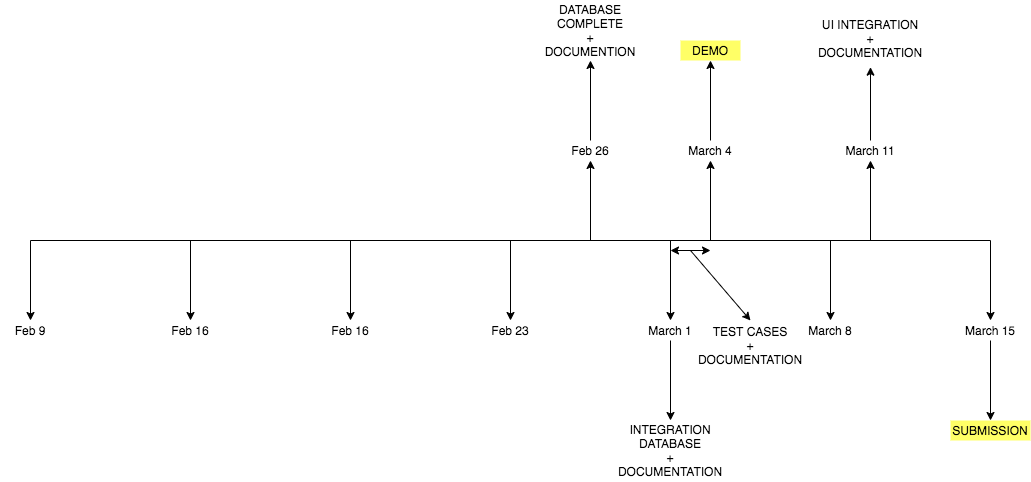
\includegraphics[scale=0.5]{timeline.png}
    \caption{Timeline}
    \label{fig:UI-1}
\end{figure}

\newpage

{\bf Date:} 26 February 2020\\
{\bf Start Time:} 19:00\\
{\bf End Time:} 21:00\\
{\bf Who:} Tiffany Ah King, Isabelle Charette, Brian Gamboc-Javiniar, Vsevolod Ivanov,\\
Chang Liu, Nolan Mckay, Nalveer Moocheet, Hoang Thuan Pham, Audrey-Laure St-Louis, Jia Ming Wei\\
{\bf Where:} LB-451 (Brazil)\\
{\bf Agenda topics discussed:} \\
(1) Documenters should review Latex and create a sample document.
(2) Coders should review JUnit and create sample unit tests.
(3) The team should meet and resolve any misunderstandings for Iteration 2 about the domain model and use cases; hear how the Coders plan to implement their assigned use case; hear what issues the Documenters have, and what content/information they need. Everyone can help create sample data as needed by the unit tests.
(4) Review the timeline overall for iteration 2, assigned tasks and deadlines
(5) Plan the Demo next week
{\bf Alternatives presented:} N/A\\
{\bf Solutions agreed upon:} \\
(1) Use the Database with GJson serializer for the model. \\
{\bf Assignments made and accepted:} \\
(1) Vsevolod will be the Organizer, Pull-Request reviewer and help QAs.\\
(2) Nolah will help to code more DB.\\
(3) Brian will continue our DB API and the Epic and merge into it more code.\\
(4) Tifany, Nalveer and Chang continue the QA of new codes.\\
(5) Hoang will finish the UI features in View and Controller.\\
(6) Jia, Audrey and Isabelle will continue the documentation.\\
{\bf Deadlines:} \\
(1) MVC Diagram and Documentation V1 19 February 2020;\\
(2) Database delivery with API and Documentation V2 26 February 2020;\\
(3) Demo, Documentation V3, Tests and Integration March 4 2020; \\
(4) UI Integration 11 March 2020. \\
(5) Submission 15 March 2020 at 21:59. \\
{\bf Follow-up actions:} Everything is advancing well, the QA needs a bit of jump-start.\\

\begin{table}[h!]
\centering
 \begin{tabular}{||l l c ||} 
 \hline
   & Task & Progress Status\\ [0.5ex] 
 \hline\hline
 1 & Suggest technological alternatives & done \\
 2 & SQlite database & done\\
 3 & SQlite database API & in progress\\
 4 & Database QA from our MVC code base & in progress\\
 5 & Retart game, UI for load/save game & in progress\\
 6 & QA of restart/load/save game controller etc., modular components & in progress\\[1ex] 
 \hline
 \end{tabular}
\caption{Follow-up }
\label{table:1}
\end{table}

\newpage

{\bf Date:} 04 March 2020\\
{\bf Start Time:} 19:15\\
{\bf End Time:} 21:00\\
{\bf Who:} Tiffany Ah King, Isabelle Charette, Brian Gamboc-Javiniar, Vsevolod Ivanov,\\
Chang Liu, Nolan Mckay, Nalveer Moocheet, Hoang Thuan Pham, Audrey-Laure St-Louis, Jia Ming Wei\\
{\bf Where:} H-831\\
{\bf Agenda topics discussed:} \\
(1) Do the demo.
(2) Discuss any issues, bugs.
{\bf Alternatives presented:} N/A\\
{\bf Solutions agreed upon:} Refactor new code.\\
{\bf Assignments made and accepted:} \\
(1) Vsevolod will be the Organizer, Pull-Request reviewer and help QAs.\\
(2) Nolah will help to code more DB.\\
(3) Brian will continue our DB API and the Epic and merge into it more code.\\
(4) Tifany, Nalveer and Chang continue the QA of new codes.\\
(5) Hoang will finalize the UI features in View and Controller.\\
(6) Jia, Audrey and Isabelle will finalize the documentation.\\
{\bf Deadlines:} \\
(1) MVC Diagram and Documentation V1 19 February 2020;\\
(2) Database delivery with API and Documentation V2 26 February 2020;\\
(3) Demo, Documentation V3, Tests and Integration March 4 2020; \\
(4) UI Integration 11 March 2020. \\
(5) Submission 15 March 2020 at 21:59. \\
{\bf Follow-up actions:} Integrate everyone work to master and continue the team effort.\\

\begin{table}[h!]
\centering
 \begin{tabular}{||l l c ||} 
 \hline
   & Task & Progress Status\\ [0.5ex] 
 \hline\hline
 1 & Suggest technological alternatives & done \\
 2 & SQlite database & done\\
 3 & SQlite database API & done\\
 4 & Database QA from our MVC code base & done\\
 5 & Retart game, UI for load/save game & done\\
 6 & QA of restart/load/save game controller etc., modular components & in progress\\[1ex]
 7 & Refactor new code & in progress\\ 
 \hline
 \end{tabular}
\caption{Follow-up }
\label{table:1}
\end{table}

\end{document}
